\documentclass[10pt]{article}
\usepackage[utf8]{inputenc}
\usepackage{listings}
\usepackage{float}
\usepackage{graphicx}
\usepackage{fullpage}
\usepackage{caption}
\usepackage{subcaption}
\usepackage{amsmath}
\usepackage{hyperref}

%\renewcommand{\thesubsection}{\arabic{subsection}}
\renewcommand{\thesubsubsection}{\alph{subsubsection}}

\title{Pattern Recognition Practical 4}
\author{Group 24: \and Maikel Withagen (s1867733) \and Steven Bosch (s1861948)}
\date{\today}
\lstset{
frame=single, 
numbers=left, 
breaklines=true, 
language=Matlab,
basicstyle=\small, 
title=\lstname
}

\renewcommand{\thesection}{Assignment \arabic{section}}
\renewcommand{\thesubsection}{\arabic{subsection}}
\begin{document}
\section{Assignment 1}
\subsection{}
Using the code given in the appendix we created the scatterplot in figure \ref{fig1.1}.

\begin{figure}[H]
 \centering
 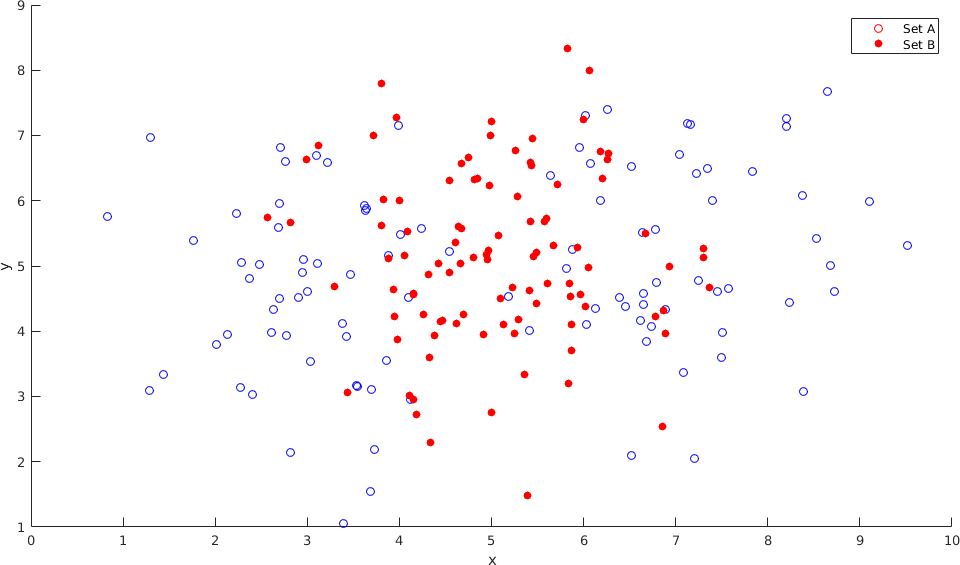
\includegraphics[width=\textwidth]{Fig1_1.png}
 \caption{Scatterplot for the two classes.}
 \label{fig1.1}
\end{figure}

The plot shows that there are at least three prototypes needed to approach a fairly well classification of these data. Two for set A, which should probably be located around $(3,4.5)$ and $(7.5, 5.5)$, and one for set B somewhere around $(5,5)$. 

\subsection{}
The code in the appendix shows our implementation of the LVQ1 algorithm. We acquired the following results for the different settings.

\subsubsection{1 Prototype for class A and 1 prototype for class B}


\section*{Appendix}
\lstinputlisting{../Code/Ass1_1.m}
\lstinputlisting{../Code/Ass1_2.m}


\maketitle
\end{document}
